% !TeX spellcheck = fr_FR
\section{\Duo}
La traductions de \Duo{} \begin{CJK*}{UTF8}{bsmi}剁\end{CJK*} fait référence au terme de cuisine \textit{émincer} qui évoque en quelque sorte un mouvement répété et une coupe utilisant une partie de la lame plus éloignée de la pointe que \Pi{}. Le mouvement lui-même est la combinaison d'une extension vers l'avant et d'une sorte de cisaillement, comme lorsqu'on utilise un gros couteau de cuisine pour émincer des herbes aromatiques ou des légumes.

Dans la tradition du \Yangjia{} \Michuan{}, \Duo{} est typiquement réalisé avec les deux bras étendus pratiquement dans l'alignement de la lame de l'épée (fig. \ref{fig:duo_full}). 


\begin{figure}[ht]
	\centering
	
	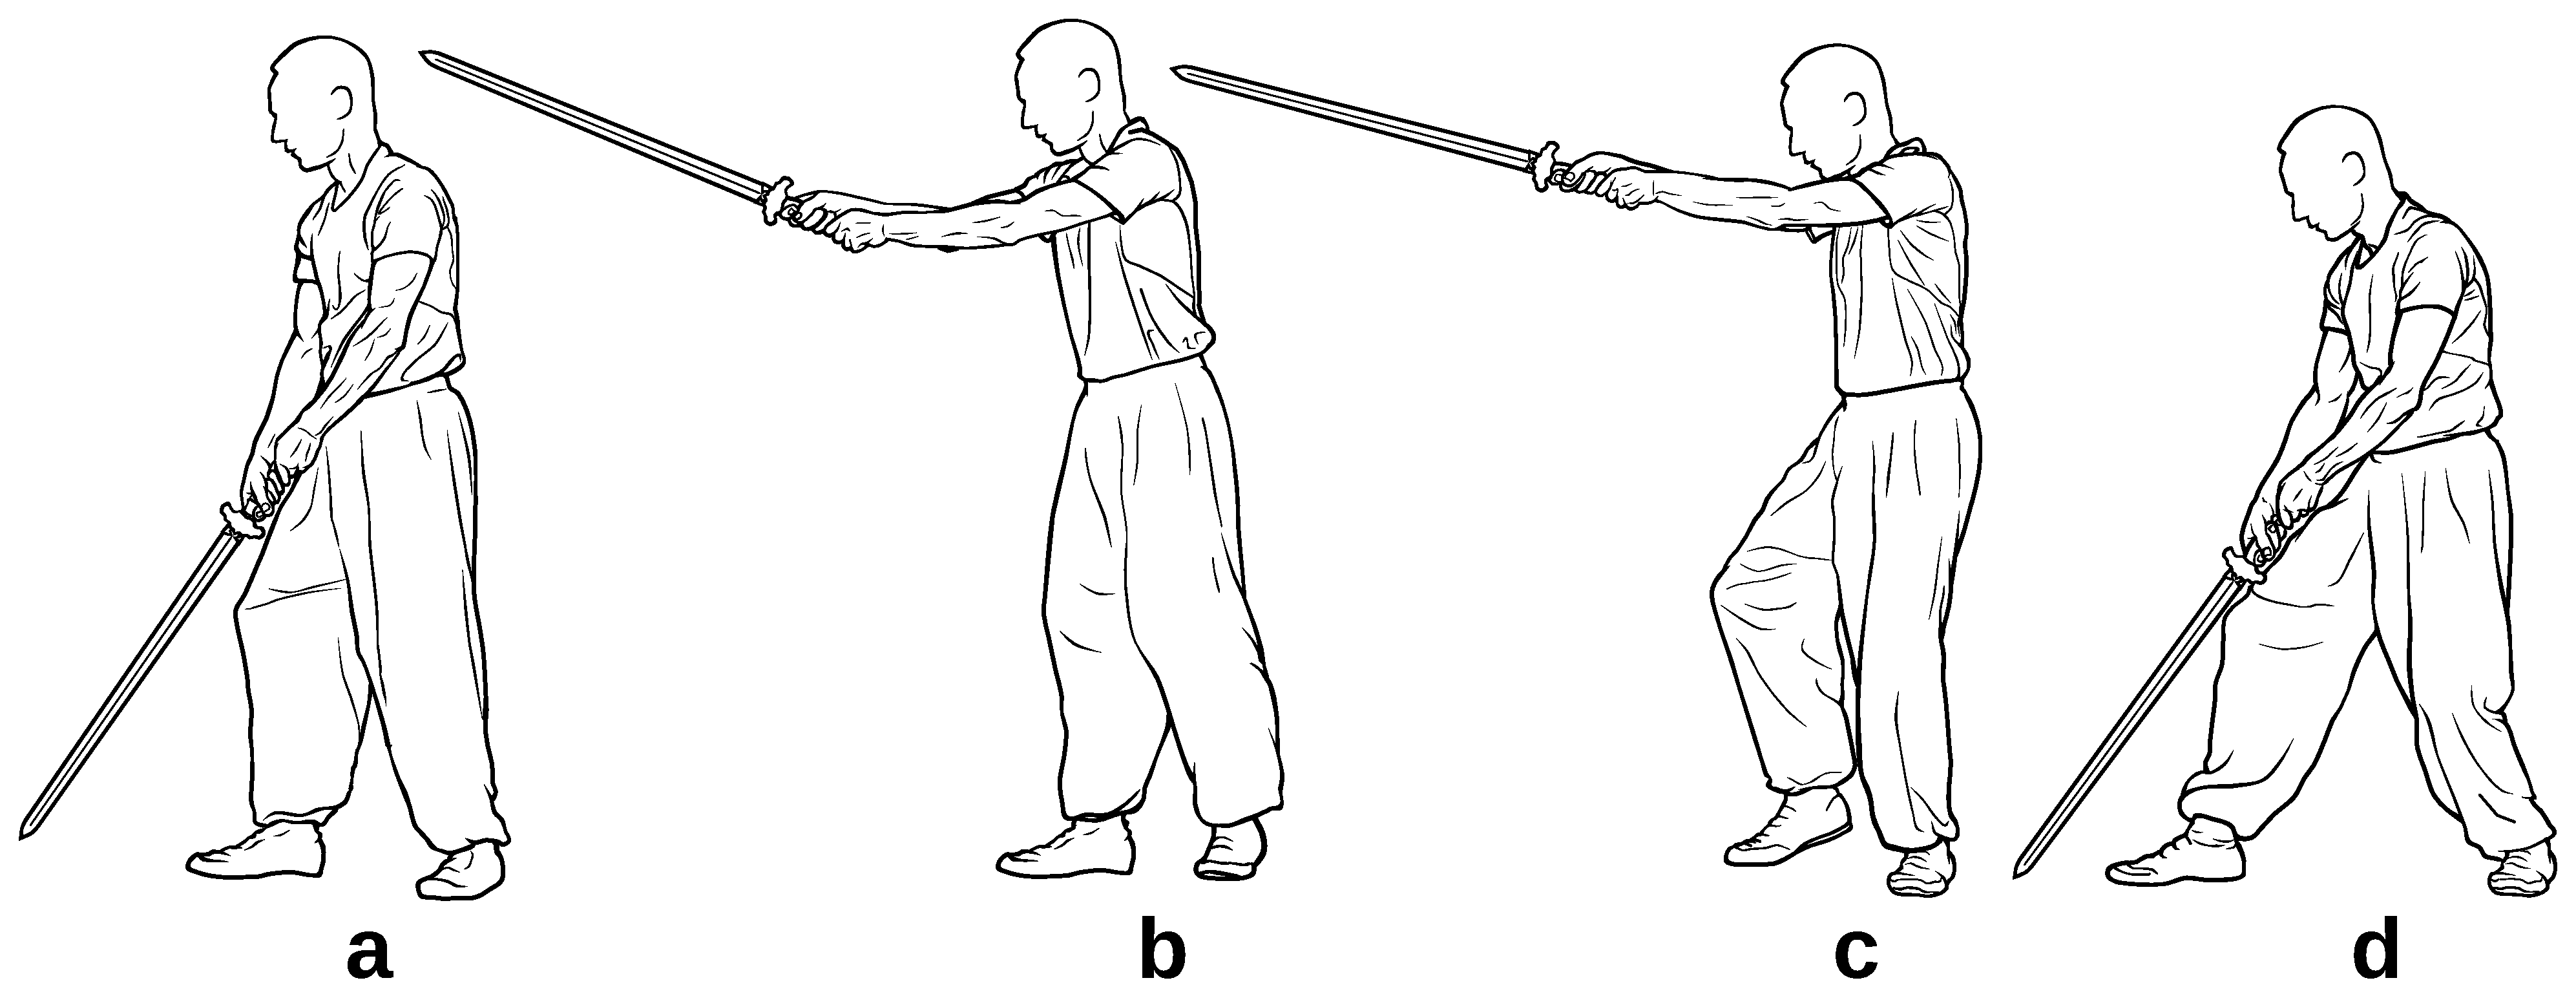
\includegraphics[width=1.00\textwidth]{../../Images/JibenJianfa/Duo/Duo.pdf}
	\caption[\Duo{} en avançant]{\Duo{} en avançant. À partir d'une garde basse (a), lever l'épée en transférant le poids sur le pied droit (b), inverser la polarité entre les mains et transférer le poids à nouveau sur le pied gauche (c), puis abaisser l'épée tout en s'enracinant dans la jambe gauche et en avançant le le pied droit.}
	\label{fig:duo_full}
\end{figure} 

Bien que les deux mains soient en contact avec la poignée, il ne faut pas confondre cette position avec une prise à deux mains de la fusée. À la montée et en avançant, la main droite tient l'épée tandis que la main gauche donne la structure et transmet la puissance naissant dans la taille en poussant sur le pommeau suivant la direction de la lame. La combinaison du rôle passif de la main droite et de l'action de la main gauche crée une polarité induisant un mouvement de l'épée perpendiculaire à l'axe du bras droit. À la descente, les rôles des deux mains sont inversés (fig. \ref{fig:duo_detail}). 

\begin{figure}[ht]
	\centering
	
	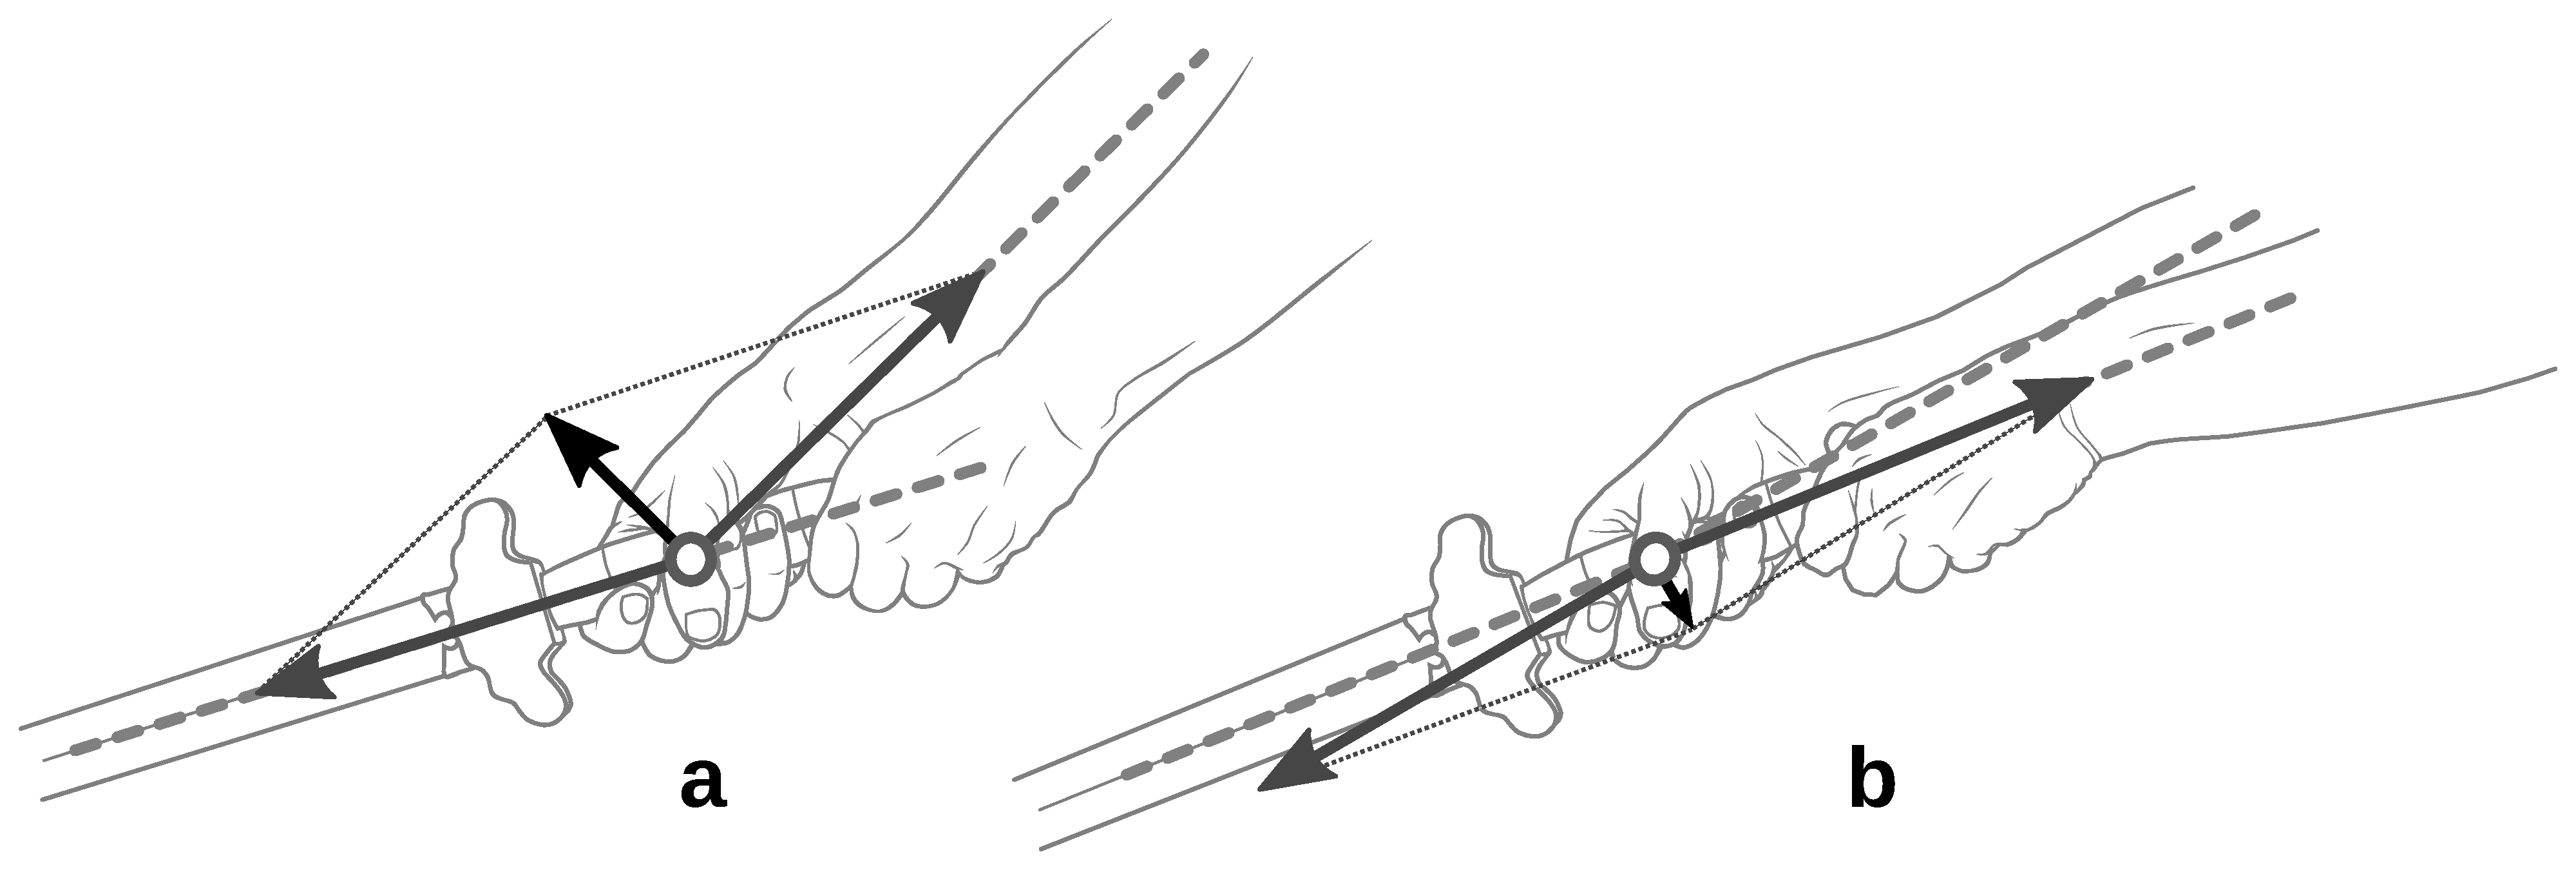
\includegraphics[width=1.00\textwidth]{../../Images/JibenJianfa/Duo/DuoDetail.pdf}
	\caption[Équilibre des forces dans le \Duo{}]{(a) Pour réaliser un \Duo{} ascendant vers l'avant, la main gauche pousse la poignée dans la direction de la pointe de la lame tandis que le bras droit équilibre passivement cette poussée. En raison de l'angle entre la direction de poussée et le bras droit, il en résulte une force perpendiculaire au bras droit qui fait monter l'épée.\\
	(b) Pour réaliser un \Duo{} descendant vers l'avant, la main droite pousse la poignée vers l'avant tandis que la main gauche la retient passivement en équilibrant la force de poussée. La force résultante, perpendiculaire à l'axe du bras gauche, tire l'épée vers le bas.
	}
	\label{fig:duo_detail}
\end{figure} 

Dans un \Duo{} montant en avançant, la force est générée par le transfert de poids de la jambe arrière à la jambe avant. Elle est transmise à l'épée par la main gauche/arrière pendant que la main droite/avant équilibre exactement et passivement cette force pour générer la technique sans effort. Une connexion effective entre la taille et l'épée permet alors l'expression explosible de la technique \Duo{}.
Cette méthode fait en quelque sorte écho aux préceptes trouvés dans le \JianJing{}  précisant que, en manipulant une épée à deux mains, la puissance est dans la taille, puis dans la main arrière, et finalement dans la main avant.

Pour \Duo{} en reculant toutefois, les mains jouent un rôle inverse : la main droite est active en montant, et passive en descendant. Une règle générale est, qu'on avance ou qu'on recule, que la main active est celle qui se trouve du même côté que le pied qu'on déplace.

Puisqu'en cuisine, les aromates et légumes sont généralement émincés en coupant vers le bas, on peut argumenter que la phase active de \Duo{} serait la phase descendante. Toutefois, l'examen attentif du mouvement réel d'un couteau de cuisine lorsqu'on émince montre que la phase active correspond en réalité à la phase ascendante de \Duo{} en avançant. La seule différence est que dans le cas du couteau, la pointe reste au contact du plan de travail tandis que la pointe de l'épée monte, mais dans les deux cas, le tranchant suit un mouvement similaire relativement à la pointe.
Il est cependant parfaitement possible d'être actif pendant les deux phases, la phase passive étant en fait le mouvement de transition entre la montée et la descente. Ainsi, \Duo{} peut tout aussi bien être un estoc ou une coupe en montant ou en descendant. Cette technique peut même, combinée à \Mo{}, une action sur la lame de l'adversaire, soit en montant pour intercepter et dévier, soit en descendant pour un froissement. 

It is worth noting at this point that, since both hands are in contact with the handle, the sword is always in line with the axis of the body. This axis is more to the left when we are on our left foot, in the low on-guard position that precedes the ascending forward phase of \Duo{}. Reciprocally, the axis is shifted to the right as we stand on our right foot after we have completed the ascending forward stage of the movement. This has strong implications on the deflect/shear application of  \Duo{} in combination with \Mo{}. Deflecting while transferring the weight to the right gently pushes the opponent's tip away, then, the descending shear naturally aims at the centre of the opponent's sword, deflecting it further to open the way for a hit while preventing any counter attack. 

\fiche{The simplest application of \Duo{} starts with a lower guard as an invitation for the opponent to prepare an attack. We can then engage and deflect with a \Duo{} before placing our riposte or we may take advantage of the explosive nature of the movement and use an offensive \Duo{} to thrust directly during the opponent's preparation.
	\Duo{} is often performed in series of two to three movements, not more to avoid predictability, as seen for the double-handed version in the \Kunlun{} form. We can usually identify three periods in these series: The first \Duo{} movement would intercept an incoming attack, either a \Pi{} or a \Hua{} cut from above or a high level \Ci{} thrust.Then, the second one will deflect the opponent's blade to open the way for the third \Duo{} thrust. Of course, this is not a fixed pattern, and the first movement can be followed by any appropriate technique depending on the circumstances. For instance, instead of deflecting, the second step may accompany the opponent's blade to control it while entering to prepare the riposte.}

Although the classic movement is done with two hands, it is also possible to perform a \Duo{} with one hand only. In this case, the heel of the right hand plays the role of the left hand and the first three fingers \textemdash{} the index and middle fingers, and the thumb \textemdash{} play the part of the right hand (figure). 

During the ascending phase, the handle of the sword is pushed forwards by the heel of the hand and simultaneously pulled by the first three fingers. Given a good structure in the on-guard position, it is then possible, even with only one hand, to swiftly and effortlessly raise the sword from a low to a high position, for thrusting or engaging.  
\fiche{When descending, the fore fingers relax their grip while the ring and little fingers are tightened to pull the handle. Some intention should be put at the base of the index to gently push the handle downwards in the forward direction. The resulting structure allows to capture and deflect the centre of the opponent's sword by shearing or to perform a powerful cut while retreating.}
The alignment of the sword is quite similar to the two-handed version, with the tip of the blade in line with the body axis. However, the structure is not as strong as in the two-handed \Duo{} and, as a result, the shearing actions are not as powerful. However, this version of the movement is useful for quickly engaging the opponent's blade or a sudden attack from a lower guard. 